\documentclass[12pt,a4paper]{article}
\usepackage[T1]{fontenc}
\usepackage{times}
\usepackage{graphicx}
\usepackage{xcolor}
\usepackage{fancyhdr}
\usepackage{natbib}
\usepackage{amssymb}
\usepackage{amsmath}
\usepackage{amsthm}
\usepackage{mathrsfs}
\usepackage{empheq}
\usepackage{bm}
\newcommand{\size}{0.22\textwidth}
\newcommand{\avg}[1]{\left<#1\right>}
\renewcommand{\avg}[1]{\left<#1\right>}
\newcommand{\Exp}[1]{\overline{\overline{#1}}}
\newcommand{\davg}[1]{\left<#1\right>_d}
\newcommand{\cavg}[1]{\left<#1\right>_c}
\newcommand{\pavg}[1]{\avg{\delta_\alpha #1}}
% \newcommand{\pnavg}[1]{n\left<#1\right>_p}

\newcommand{\avgcond}[1]{\left<#1\right>}
\renewcommand{\avgcond}[1]{\overline{#1}}
\newcommand{\condavg}[2]{\overline{#1}^{#2}}
\newcommand{\ravg}[1]{\avgcond{#1}^\textbf{r}}
\newcommand{\Tavg}[1]{\avgcond{#1}^T}
\newcommand{\Xavg}[1]{\avgcond{#1}^X}
\newcommand{\TXavg}[1]{\Tavg{\Xavg{#1}}}
\newcommand{\kavg}[1]{\avgcond{#1}^k}
\newcommand{\Iavg}[1]{\avgcond{#1}^I}
\newcommand{\pnnavg}[1]{\avgcond{#1}^{p}}
\newcommand{\pnavg}[1]{n_p\pnnavg{#1}}
\newcommand{\oneavg}[1]{\avgcond{#1}^1}
\newcommand{\twoavg}[1]{\avgcond{#1}^2}
\newcommand{\smallavg}[2]{\avgcond{#1}^{#2}}
\newcommand{\sym}[1]{\text{Sym}\left[#1\right]}

\newcommand{\nstavg}[1]{\overline{#1}^{nst}}
\newcommand{\nstrelavg}[1]{\overline{#1}^{nst}_{rel}}
\newcommand{\mavg}[1]{\left<#1\right>_m}
\newcommand{\gavg}[2][\gamma]{\left<#2\right>_{#1}}
\newcommand{\partials}[1]{\partial_{i_1}\partial_{i_2}\ldots\partial{i_{#1}}}
\newcommand{\partialp}[2]{ \prod_{m=#1}^{#2} \partial_{i_m}}
\newcommand{\hatpartialp}[2]{ \prod_{m=#1}^{#2} \hat{\partial}_{j_m}}
\newcommand{\hatpartialpi}[2]{ \prod_{m=#1}^{#2} \hat{\partial}_{i_m}}
\newcommand{\pri}[2]{ \prod_{m=#1}^{#2} r_{i_m}}
\newcommand{\prj}[2]{ \prod_{m=#1}^{#2} r_{j_m}}

\newcommand{\grad}{\mathbf{\nabla}}
\renewcommand{\div}{\mathbf{\nabla}\cdot}
\newcommand{\gradI}{\mathbf{\nabla}_{||}}
\newcommand{\divI}{\mathbf{\nabla}_{||}\cdot}

\newcommand{\ddt}{\frac{d}{dt}}
% \renewcommand{\ddt}{d_t}
\newcommand{\pddt}{\frac{\partial}{\partial t}}
\newcommand{\Dt}{D_t}
\newcommand{\pddx}{\frac{\partial}{\partial \textbf{x}}}
\newcommand{\pddr}{\frac{\partial}{\partial \textbf{r}}}
\newcommand{\pddy}{\frac{\partial}{\partial \textbf{y}}}
\newcommand{\pddw}{\frac{\partial}{\partial \textbf{w}}}
\renewcommand{\pddx}{{\partial_\textbf{x}}}
\renewcommand{\pddr}{{\partial_\textbf{r}}}
\renewcommand{\pddy}{{\partial_\textbf{y}}}
\renewcommand{\pddw}{{\partial_\textbf{w}}}
\newcommand{\pdda}{\partial_a}
\renewcommand{\pddt}{\partial_t}
\newcommand{\norm}[1]{\hat{#1}}
\newcommand{\Jump}[1]{\llbracket #1 \rrbracket \cdot \textbf{n}_k }
\renewcommand{\Jump}[1]{\sum_{k=d,f} \left[#1\right] \cdot \textbf{n}_k }

\newcommand{\intO}[1]{\int_{V_\alpha} #1 dV}
% \renewcommand{\intO}[1]{ ( #1 )_{\Omega}}
\newcommand{\intS}[1]{\oint_{S_\alpha} #1 dS}
% \renewcommand{\intS}[1]{ ( #1 )_{\Sigma}}
\newcommand{\pOavg}[1]{\pavg{\intO{#1}}}
\newcommand{\pSavg}[1]{\pavg{\intS{#1}}}
\newcommand{\pMavg}[1]{\mathscr{M}\!\!\left[#1\right]}
\newcommand{\pMOavg}[1]{\mathscr{M}_\Omega\!\!\left[#1\right]}
\newcommand{\pMSavg}[1]{\mathscr{M}_\Sigma\!\!\left[#1\right]}
\newcommand{\CC}{\mathscr{C}}
\newcommand{\PP}{\mathscr{P}}
\newcommand{\FF}{\mathscr{F}}

%%% Utiliser pour les commentaires
\newcommand{\JL}[1]{\color{red}#1\color{black}}
\newcommand{\DL}[1]{\color{green}#1\color{black}}
\newcommand{\tb}[1]{\color{blue}#1\color{black}}
% \renewcommand{\alpha}{}
% \renewcommand{\tb}[1]{}

\renewcommand{\size}[1]{0.3\textwidth}
\newcommand{\expo}[2][n]{\frac{(-1)^#1}{#1!} \partialp{1}{#1} \pavg{\int_{\Omega_\alpha} \pri{1}{#1}#2 d\Omega}}
\newcommand{\expoU}[2][n]{\frac{(-1)^#1}{#1!} \partialp{1}{#1} \pavg{\textbf{u}_\alpha\int_{\Omega_\alpha} \pri{1}{#1}#2 d\Omega}}
\newcommand{\expoS}[2][n]{\frac{(-1)^#1}{#1!} \partialp{1}{#1} \pavg{\int_{\Gamma_\alpha} \pri{1}{#1}#2 d\Sigma}}

% \newcommand{\numref}[1]{\ref{#1}}
% \renewcommand{\ref}[1]{\autoref{#1}}

% FORMAT OF PAGE
\addtolength{\textheight}{4.5cm}
\addtolength{\topmargin}{-1.5cm}
\addtolength{\footskip}{0cm}
\addtolength{\textwidth}{5cm}
\addtolength{\evensidemargin}{-2.5cm}
\addtolength{\oddsidemargin}{-2.5cm}

\definecolor{mygray}{gray}{0.6}
\renewcommand\refname{\textbf{\large References}}


\begin{document}

\pagestyle{fancy}
\fancyhf{}

\lhead{\textcolor{mygray}{12th International Conference on Multiphase flow}}
\rhead{\textcolor{mygray}{ICMF 2025, Toulouse, France, May 12-16, 2025}}
\lfoot{}
\cfoot{}
\rfoot{}

% TITLE IN CAPITAL LETTERS
\begin{center}
{\large {\bf Theoretical calculation of the droplet induced agitation (or pseudoturbulence) in mono disperse buoyant emulsions for low inertia and dilute regimes}}
\vspace{10pt}

% AUTHORS

\underline{Nicolas Fintzi}$^1$, Jean-Lou Pierson$^1$, and St\'ephane Popinet$^2$\\
% AFFILIATIONS
{\it
$^1$IFP Energies Nouvelles, Solaize, 69360, France, nicolas.fintzi@ifpen.fr, jean-lou.pierson@ifpen.fr\\
$^2$Sorbonne Universit\'e, Institut Jean le Rond $\partial$'Alembert, 75252 Paris, France, popinet@basilisk.fr\\
%$^3$Affiliation of third author: University, School, Department, Institute, City, Country, E-mail\\
}
\end{center}

\vspace{10pt}
\noindent{\bf {\large Abstract}}:\\
Buoyancy-driven droplet flows are encountered in many chemical engineering processes such as gravity separators and liquid-liquid extractors. 
The usual engineering practice to model such facilities is to use the averaged Navier-Stokes equations. 
The present work focuses on the velocity fluctuations tensor, also known as the \textit{Reynolds stress} tensor, or Pseudo-turbulent tensor, which is a crucial closure term in these equations.
Formally, this stress is defined as $\avg{ \textbf{u}' \textbf{u}'}_f$, where $\textbf{u}'$ is the fluid velocity fluctuation, and $\avg{\ldots}_f$ denotes an ensemble average procedure applied over the continuous phase. 
The \textit{Reynolds stress} can be separated into two contributions : (1) The agitation generated due to the averaged wakes around the particles; (2) All other sources of fluctuations, such as those generated through particle interactions, and single-phase turbulence. % \cite{du2022analysis}.
This study only considers the first contribution. 
Specifically we compute $\avg{ \textbf{u}' \textbf{u}'}_f$, for buoyant rising droplets in an otherwise quiescent fluid. 
The derivation is restricted to spherical droplets (of radius $a$), at small particle Reynolds number, and low particle volume fraction ($\phi$). 
    \vspace{10pt}

\noindent{{\bf Keywords}}: Reynolds stress, pseudoturbulence, averaged equations, dispersed multiphase flows, droplets. 

\vspace{10pt}

% \noindent{\bf {\large Problematic}}:

For buoyant inviscid bubbly flows under the dilute assumption, it is known since the study of \cite{van1982bubble} that the \textit{Reynolds stress} can be written as
\begin{equation}
    \avg{\textbf{u}'\textbf{u}'}_f (\textbf{x})
    \approx
    n_p \int_{|\textbf{r}| > a}\textbf{v}\textbf{v}  d\textbf{r}
    = \phi \left(\frac{3}{20} U^2\textbf{I} + \frac{1}{20} \textbf{UU} \right),
    % \\+\underbrace{\int_{\mathbb{R}^3} \textbf{R} P_{f}^1(\textbf{x},\textbf{r}) d\textbf{r}}_\text{(2)}
    % - \phi_f \textbf{u}_f\textbf{u}_f,
    \label{eq1}
\end{equation}
where $n_p$ is the number of particles per unit of volume, $\textbf{U}$ is the averaged particle velocity, and $\textbf{v}$ is the disturbance velocity field of an isolated particle. 
The integral in Equation (\ref{eq1}) can be computed since $\textbf{v} \sim \mathcal{O}(r^{-3})$, with $r =|\textbf{r}|$ in the case of potential flows. 
However, the disturbance velocity field of a translating droplet in Stokes flows (see Figure \ref{fig:wake} (left)) decays as $\sim \mathcal{O}(r^{-1})$. 
Therefore, the integral in Equation (\ref{eq1}) cannot be computed for Stokes flows. 
This is the main reason why no theoretical model exists for $\avg{\textbf{u}'\textbf{u}'}_f$ in the limit of low Reynolds numbers. 
% \vspace{10pt}

% \noindent{\bf {\large Theoritical solution with The Nearest Particle Statistics}}:
 
To bypass the problem of divergent integrals we make use of the  \textit{Nearest Particle Statistics} framework recently revisited by \cite{zhang2021ensemble}. 
In this context we can express the \textit{Reynolds stress} in terms of nearest-particles averaged quantities, which yields
\begin{equation}
    \avg{\textbf{u}'\textbf{u}'}_f(\textbf{x},t)
    \approx
    \int_{r >a}  \textbf{v}_\text{nst}  \textbf{v}_\text{nst} P_\text{nst}^f(\textbf{r}|\textbf{x},t) d\textbf{r}.
    \label{eq:eq2}
\end{equation}
Where $P_\text{nst}^f(\textbf{r}|\textbf{x},t)$ is the probability that the nearest particle's center of mass is located at \textbf{r}, conditionally on the point \textbf{x} being occupied by the continuous phase.
And $\textbf{v}_\text{nst}$ is the disturbance velocity field evaluated at a point \textbf{x} in the continuous phase, knowing the nearest particle center of mass is at location \textbf{r}. 
In the homogeneous and dilute regime $P_\text{nst}^f(\textbf{r}|\textbf{x},t) = n_p e^{- \phi [(r/a)^3 - 8]}$ \cite{zhang2021ensemble}.
Under this hypothesis, and neglecting the effect of inertia, it is possible to compute $\textbf{v}_\text{nst}$ by solving the \textit{nearest neighbor conditionally averaged} Stokes equations \cite{zhang2021ensemble}. 
The rapid decay of $P_\text{nst}^f$ at large $r$ enables us to compute the integral of the disturbance velocity fields, even in low inertia and dilute regimes. 
Taking the trace of (2) and carrying the integration, provides the expression for the trace of the Reynolds stress, namely,
\begin{equation}
    \avg{\textbf{u}'\cdot \textbf{u}'}_f/3
    = \frac{(2+3\lambda)^2}{(\lambda+1)^2}\frac{\Gamma(1/3)}{24} 
        \phi^{2/3}
        (\textbf{u}_pf\cdot \textbf{u}_{pf})
        + \mathcal{O}(\phi),
        \label{eq:results}
\end{equation}
where $\Gamma(z) = \int_0^\infty t^{z-1} e^{-t} dt$ is the Gamma function, with $\Gamma(1/3)= 2.678$, $\lambda$ is the viscosity ratio between the dispersed and continuous phase, and $\textbf{u}_{pf}$ is the relative averaged phase velocity. 
\begin{figure}[h!]
    \centering
    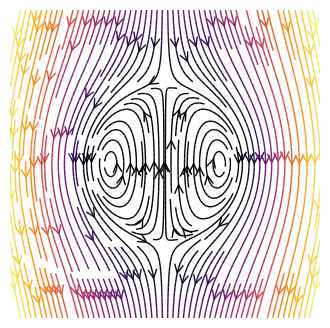
\includegraphics[height=0.25\textwidth]{image/Rising_Stokes.png}
    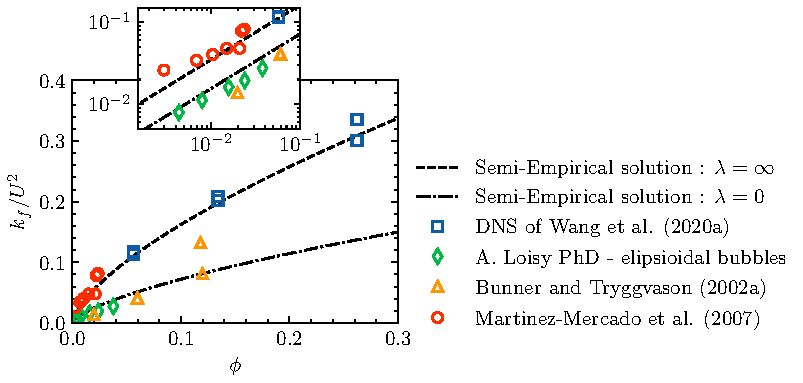
\includegraphics[height=0.3\textwidth]{image/HOMOGENEOUS_final/CA/KFliterature.pdf}
    \caption{\small
        (left) Streamlines of a translating droplet in Stokes flow. 
            (right) Dimensionless continuous phase pseudo turbulent energy, $k_f/U^2 = \avg{\textbf{u}'_y\cdot\textbf{u}'_y}_f/ |\textbf{u}_{pf}|^2$ in terms of the volume fraction $\phi$.
            (Symbols) DNS and experimental results of: 
            ($\pmb\square$)  Particle-resolved DNS
            of fixed solid spherical particle assemblies at $20< Re < 100$  by \cite{wang2021numerical}; 
            ($\pmb\lozenge$) DNS of rising deformable bubbles at $Re \approx 30$ \cite{loisy2016direct}
            ($\pmb\triangle$) DNS of rising spherical bubbles by \cite{bunner2002dynamics}. 
            ($\pmb\bigcirc$) Experiment of rising spherical bubbles in water by \cite{martinez2007measurement} at $Re \approx 30$. 
            (dot dashed lines) Semi-empirical formula (\ref{eq:semi-emprical}) at $Re \approx 30$ with $\lambda = 0$. 
            (dashed lines)  Semi-empirical formula (\ref{eq:semi-emprical}) at $Re \approx 30$ with $\lambda = \infty$.
            }
    \label{fig:wake}
\end{figure}

Direct Numerical Simulations (DNS) of rising buoyant emulsions have also been performed (with the code \texttt{http://basilisk.fr}) for $\lambda = 0.1,1,10$. 
Based on the numerical results we could validate (2) by direct comparison, and extend the domain of validity of this closure to finite Reynolds number $Re$ and higher $\phi$. 
We propose the following formula fitted on the numerical results: 
\begin{equation}
    \avg{\textbf{u}'_y\cdot \textbf{u}'_y}_f
    =
    \avg{\textbf{u}'_y\cdot \textbf{u}'_y}_f^{Re = 0}
    \left(e^{-Re} +1\right)/2. 
    \label{eq:semi-emprical}
\end{equation}
As can be observed on Figure (\ref{fig:wake}), Equation (3) is in very good agreement with both, experimental and numerical results of the literature.  
In conclusion, we developed a semi-empirical \textit{Reynolds stress} model derived in the low-inertia and dilute limit for arbitrary $\lambda$, and extended it to account for finite inertial effects using DNS data.

 

\bibliographystyle{abbrv}
\bibliography{Bib/bib_bulles.bib}
\end{document}

